\documentclass{beamer}

\usepackage{beamerthemesplit}
\usepackage{verbatim}

\usepackage{xcolor}

\definecolor{gold}{rgb}{1.,0.84,0.}
\definecolor{brightred}{rgb}{1.,0.4,0.4}
\definecolor{mygray}{RGB}{200,200,200}
\definecolor{lightsteelblue}{RGB}{176,196,222}
\definecolor{lightskyblue}{RGB}{135,206,250}
\definecolor{cadetblue}{RGB}{95,158,160}

\usetheme{default}
\usecolortheme{mule}

\usefonttheme{serif}

%\DeclareGraphicsExtensions{.pdf,.png,.jpg}

\newcommand{\snr}{$S/N$}
\newcommand{\snT}{$(S/N)_{\textrm{size}}$}
%\newcommand{\snT}{$\left( \frac{S}{N}\right)_{\textrm{size}}$}
\newcommand{\snflux}{$(S/N)_{\textrm{flux}}$}
%\newcommand{\snflux}{$\left( \frac{S}{N}\right)_{\textrm{flux}}$}

\newcommand{\lensfit}{\texttt{LENSFIT}}
\newcommand{\numba}{\texttt{Numba}}
\newcommand{\python}{\texttt{Python}}
\newcommand{\ngmix}{\texttt{ngmix}}
\newcommand{\shear}{{\bf g}}
\newcommand{\redmapper}{redMaPPer}
\newcommand{\est}{$e$}
\newcommand{\mest}{e}

\newcommand{\mcalR}{$R$}
\newcommand{\mcalRpsf}{$R^{p}$}
\newcommand{\mcalRS}{$R_{S}$}

\newcommand{\prelim}{{\bf{\it Preliminary}}}



\title{Update on Metacalibration for Weak Lensing Shear Measurement}
\author{Erin Sheldon}
\institute{Brookhaven National Laboratory}

% http://texblog.net/latex-archive/plaintex/beamer-footline-frame-number/
% to add the page (frame ) number and not screw up the bottom line
% works for split themes?
\expandafter\def\expandafter\insertshorttitle\expandafter{%
      \insertshorttitle\hfill%
        \insertframenumber\,/\,\inserttotalframenumber}

% suppress navigation bar
\beamertemplatenavigationsymbolsempty
\setbeamertemplate{footline}{}

\begin{document}

\frame{\titlepage}


\setbeamertemplate{background canvas}[vertical shading][bottom=mgray,top=mblack]

\frame
{
    \frametitle{Outline}

    \setbeamerfont*{itemize/enumerate body}{size=\Large}
    \setbeamerfont*{itemize/enumerate subbody}{parent=itemize/enumerate body}
    \setbeamerfont*{itemize/enumerate subsubbody}{parent=itemize/enumerate body}
 
    \begin{itemize}

        %\item The Primary Goal is to Study Dark Energy
        \item Metacalibration

        \item Selection Effects

        \item Additive Bias correction

    \end{itemize}

}

\frame
{
    \frametitle{Shear Accuracy Requirements}

    \setbeamerfont*{itemize/enumerate body}{size=\Large}
    \setbeamerfont*{itemize/enumerate subbody}{parent=itemize/enumerate body}
    \setbeamerfont*{itemize/enumerate subsubbody}{parent=itemize/enumerate body}
 
    \begin{itemize}

        \item In order to measure the Dark Energy equation of state
            to the desired accuracy for DES/LSST, we must measure
            shear with exquisite accuracy.

        \item LSST Requirements
            \begin{itemize}
                \item Multiplicative errors: {\color{gold} $\Delta \gamma/\gamma \lesssim 0.001$}
                \item Additive errors: {\color{brightred} $\Delta \gamma \lesssim 0.0001$}
            \end{itemize}


    \end{itemize}

}



\frame
{
    \frametitle{Metacalibration Idea from Eric Huff}

    \setbeamerfont*{itemize/enumerate body}{size=\normalsize}
    \setbeamerfont*{itemize/enumerate subbody}{parent=itemize/enumerate body}
    \setbeamerfont*{itemize/enumerate subsubbody}{parent=itemize/enumerate body}
 
    \begin{itemize}

        \item Say we have a biased shear estimator {\color{gold} $e$}.  Then we can write
            {\color{gold}
                \begin{align} \label{eq:Eexpand}
                    \mest(\gamma) &= \mest|_{\gamma=0} + \gamma ~ \frac{ \partial \mest }{ \partial \gamma }\bigg|_{\gamma=0}  + ... \\
                                  &\approx e^{psf} R^{PSF} + \gamma R
                \end{align}
            } 
        \item Use image manipulation to estimate the derivative of the
            estimator with respect to shear
            {\color{gold}
                \begin{equation}
                    R = \frac{\mest(+\Delta\gamma) - \mest(-\Delta\gamma)}{2 \Delta \gamma} \nonumber 
                \end{equation}
            }
            \begin{itemize}
                \item Deconvolve the PSF
                \item Shear the image by a small amount
                \item Reconvolve by the PSF.  Use a slightly larger PSF to suppress
                    the noise amplification
            \end{itemize}


    \end{itemize}

}

\frame
{
    \frametitle{Metacalibration Idea from Eric Huff}

    \setbeamerfont*{itemize/enumerate body}{size=\Large}
    \setbeamerfont*{itemize/enumerate subbody}{parent=itemize/enumerate body}
    \setbeamerfont*{itemize/enumerate subsubbody}{parent=itemize/enumerate body}
 
    \begin{itemize}
        
        \item Corrects for modeling biases

        \item Corrects for {\em ordinary} noise-related biases

        \item Works well at high shear.

    \end{itemize}

}



\frame
{
    \frametitle{Correlated Noise}

    \setbeamerfont*{itemize/enumerate body}{size=\large}
    \setbeamerfont*{itemize/enumerate subbody}{parent=itemize/enumerate body}
    \setbeamerfont*{itemize/enumerate subsubbody}{parent=itemize/enumerate body}
 
    \begin{itemize}

        \item These convolutions and shears result in {\em {\color{gold}
            correlated noise}} Last talk I showed how to correct for this

        \item Since then I have put the last pieces together
            \begin{itemize}
                \item Selection effects
                \item Additive bias 
            \end{itemize}

    \end{itemize}

}

\frame
{
    \frametitle{Selection Effects}


    \begin{itemize}

        \item  Applying a selection to objects, for example on the signal-to-noise
            ratio \snr, can indirectly select the shapes of galaxies and result
            in a biased shear recover.

        \item For example, putting a threshold on \snr\ tends to select less
            elliptical galaxies.

    \end{itemize}

}
\frame
{
    \frametitle{Selection Effects}

    \setbeamerfont*{itemize/enumerate body}{size=\scriptsize}
    \setbeamerfont*{itemize/enumerate subbody}{parent=itemize/enumerate body}
    \setbeamerfont*{itemize/enumerate subsubbody}{parent=itemize/enumerate body}
 
    \begin{itemize}


        \item The mean shape given selection can be written as

            \begin{align}
                \langle \mest \rangle = \int S(\mest)~P(\mest)~\mest~d\mest,
            \end{align}

            where $P(e)$ is the probability distribution of ellipticities
            and $S(e)$ is the probability of selection.

        \item The response is then

            \begin{align}
                \frac{\partial \langle \mest \rangle}{\partial \gamma}\bigg|_{\gamma=0} 
                &= \int \frac{\partial S(\mest) P(\mest) \mest  }{\partial \gamma}\bigg|_{\gamma=0} d\mest \nonumber \\
                &= \int \left[ S(\mest) \frac{\partial  P(\mest) \mest  }{\partial \gamma}\bigg|_{\gamma=0} + \mest P(\mest) \frac{\partial S(\mest)}{\partial \gamma}\bigg|_{\gamma=0} \right] d\mest \\
                %&= \langle R \rangle + \int \mest P(\mest) \frac{\partial S(\mest)}{\partial \gamma}\bigg|_{\gamma=0} d\mest \nonumber \\
            \end{align}

            The first term is the response \mcalR\ we derived before, with
            selections based on the unsheared object parameters.  The second
            term is the response of the ellipticity to selections.  We can
            approximate the derivative using a finite difference:

            \begin{align}
                \frac{\partial \langle \mest \rangle}{\partial \gamma}\bigg|_{\gamma=0}
                &\approx
                \langle \mbox{\mcalR} \rangle + \int \mest~P(\mest) \left[ \frac{ S^+ - S^- }{\Delta \gamma}\right] d\mest,
            \end{align}

    \end{itemize}

}

\frame
{
    \frametitle{Selection Effects}

    \setbeamerfont*{itemize/enumerate body}{size=\scriptsize}
    \setbeamerfont*{itemize/enumerate subbody}{parent=itemize/enumerate body}
    \setbeamerfont*{itemize/enumerate subsubbody}{parent=itemize/enumerate body}
 
    \begin{itemize}

        \item Continuing...

            \begin{align}
                \frac{\partial \langle \mest \rangle}{\partial \gamma}\bigg|_{\gamma=0}
                &\approx
                \langle \mbox{\mcalR} \rangle + \int \mest~P(\mest) \left[ \frac{ S^+ - S^- }{\Delta \gamma}\right] d\mest,
            \end{align}

        \item  We can thus rewrite this in terms of the mean ellipticity when
            selections are based on the sheared parameters:

            \begin{align}
                \frac{\partial \langle \mest \rangle}{\partial \gamma}\bigg|_{\gamma=0} &\approx
                \langle R \rangle + \frac{\langle \mest \rangle^{S+} - \langle \mest \rangle^{S-}}{\Delta \gamma} \nonumber \\
                &\equiv \langle R \rangle + \langle \mbox{\mcalRS} \rangle,
            \end{align}

    \end{itemize}

}

\frame
{
    \frametitle{\snr\ thresholds}
 
    Select objects with \snr\ greater than some threshold.

    \begin{columns}
        \begin{column}{0.5\textwidth}    

            \begin{center}
                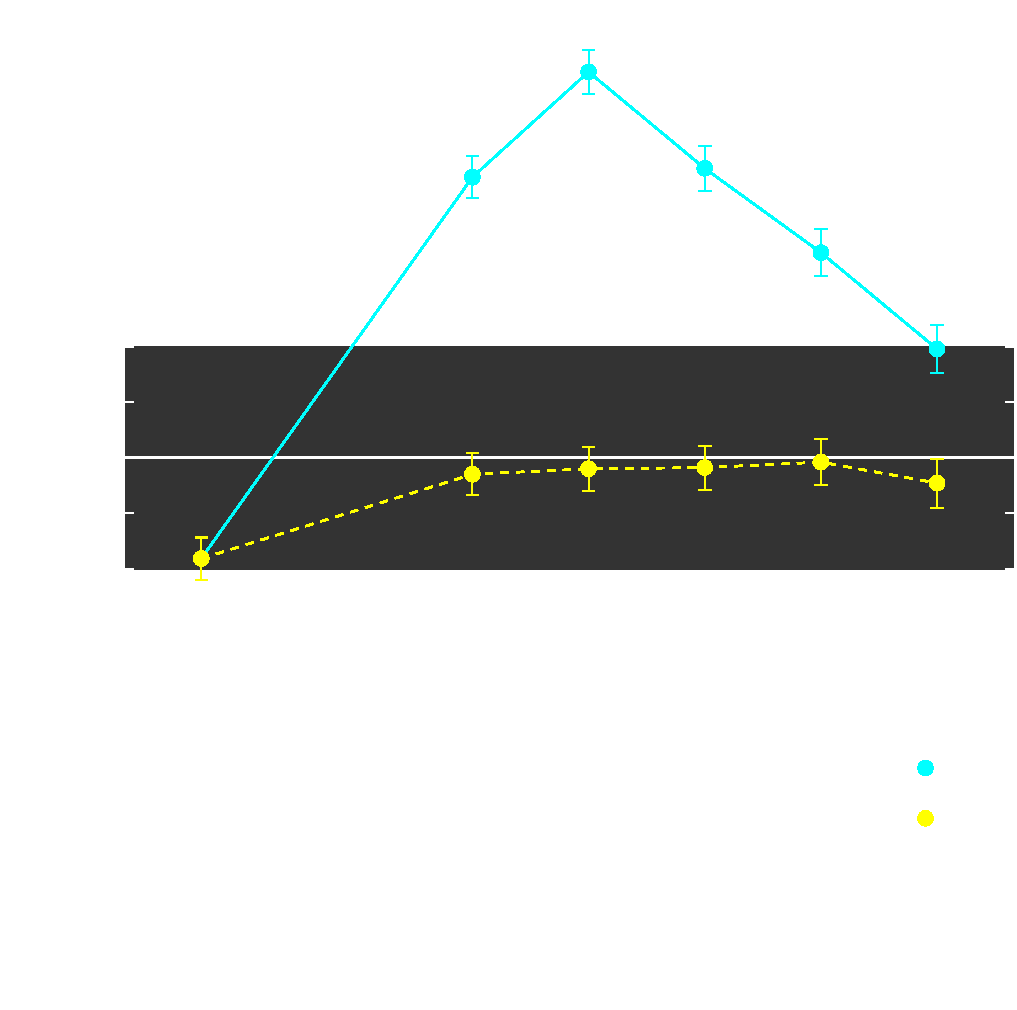
\includegraphics[width=\textwidth]{m-select-bias-thresh-inv.pdf}
                \newline
            \end{center}
        \end{column}
        \begin{column}{0.5\textwidth}
            \begin{center}
                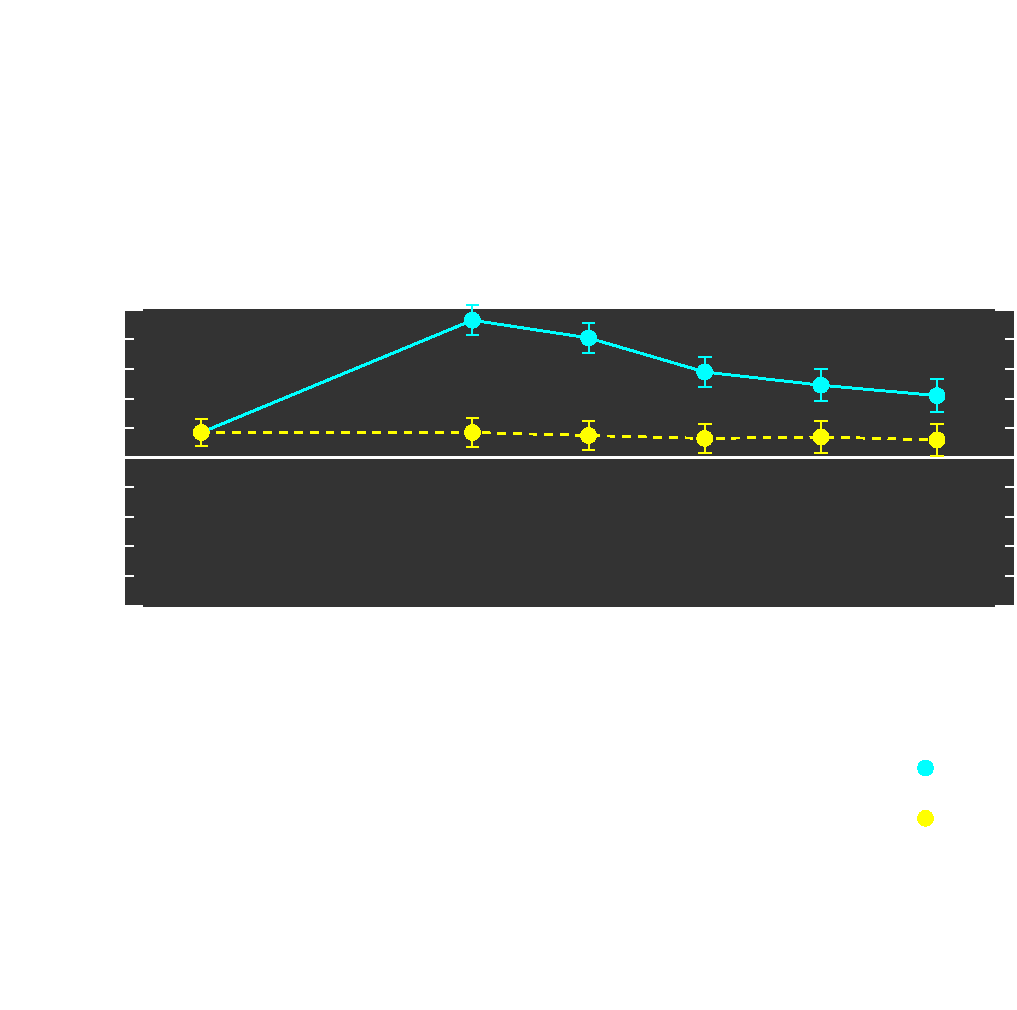
\includegraphics[width=\textwidth]{c-select-bias-thresh-inv.pdf}
                \newline
            \end{center}
        \end{column}
    \end{columns}


}

\frame
{
    \frametitle{\snr\ ranges}
 
    Select objects with \snr\ within some range.  Split into 3 equal number bins

    \begin{columns}
        \begin{column}{0.5\textwidth}    

            \begin{center}
                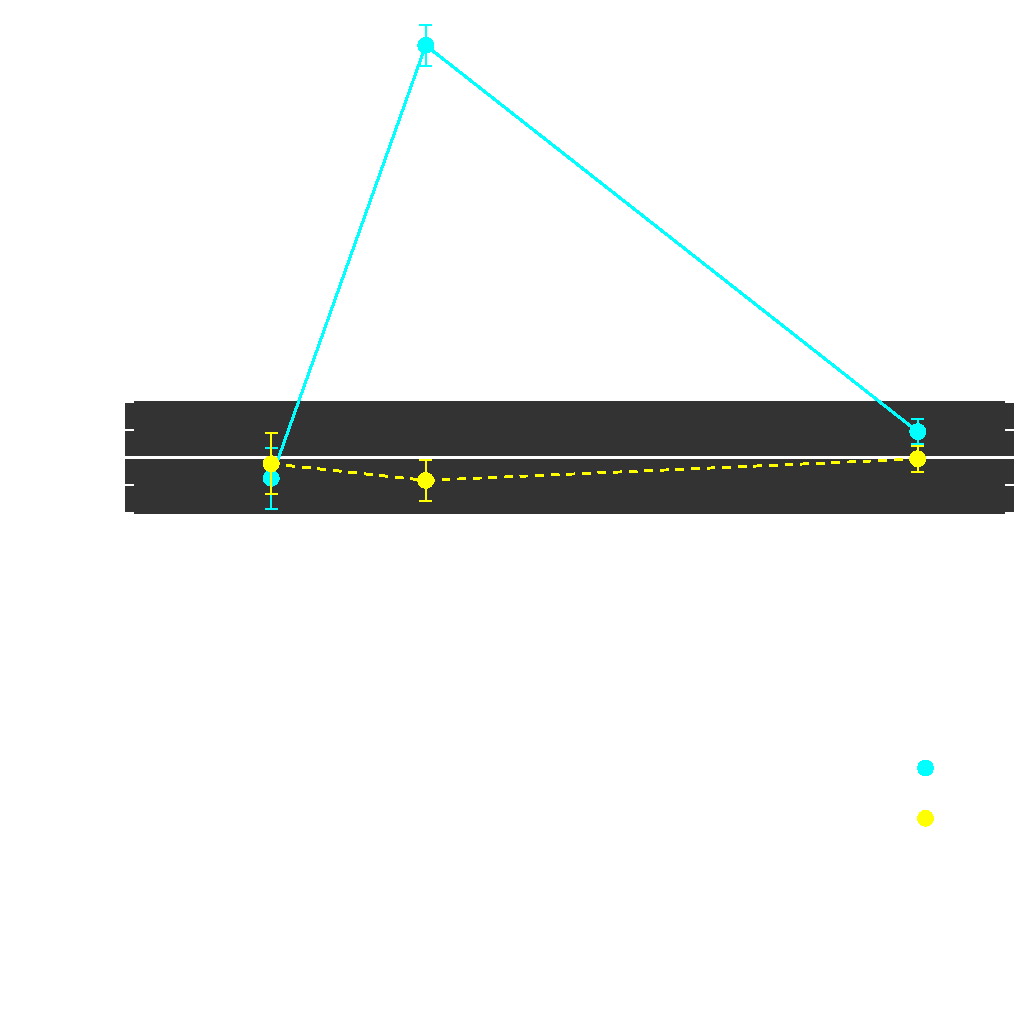
\includegraphics[width=\textwidth]{m-select-bias-range-inv.pdf}
                \newline
            \end{center}
        \end{column}
        \begin{column}{0.5\textwidth}
            \begin{center}
                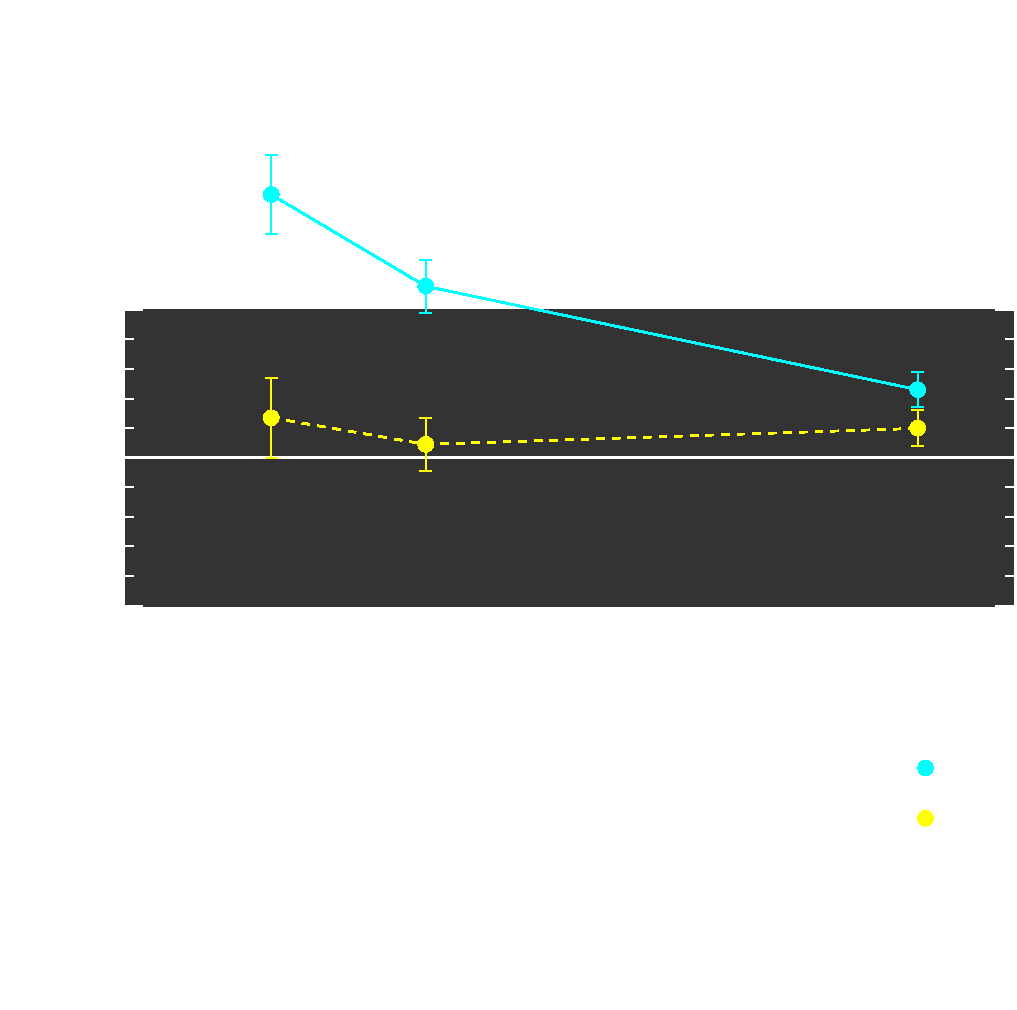
\includegraphics[width=\textwidth]{c-select-bias-range-inv.pdf}
                \newline
            \end{center}
        \end{column}
    \end{columns}


}




\end{document}
